\documentclass[
size=10pt,
paper=screen,
mode=present,
display=slidesnotes,
style=mc,
nohandoutpagebreaks,
%pauseslide,
fleqn,
clock,
,draft
]{powerdot}

\usepackage[utf8]{inputenc}
%\usepackage{polski}
\usepackage[english]{babel}
\usepackage{pstricks}
\usepackage{color}
\usepackage{xcolor}
\usepackage{tcolorbox}
\usepackage{import}
\usepackage{pstricks-add}
\usepackage{pst-grad}
\usepackage{pst-text}
\usepackage{pst-coil}
\usepackage{pst-node}
\usepackage{pst-plot}
\usepackage{array}
\usepackage{amsmath}
\usepackage{amssymb}
\usepackage{multirow}
\usepackage{graphicx}
\usepackage{verbatim}
\usepackage{fancyvrb}
\usepackage{hyperref}
\hypersetup{colorlinks=true, urlcolor=pdcolor4}
\usepackage{tikz}
\usepackage{tikz-3dplot}
\usetikzlibrary{positioning,arrows,fadings,decorations.pathreplacing,decorations.pathmorphing,decorations.markings,shapes,backgrounds,snakes}
\tikzstyle{common} = [draw, ultra thick, text centered, inner sep = 0pt, outer sep = 0pt]

\tikzstyle{filled}[pdcolor1]    = [common, color = pdcolor2, fill = #1]
\tikzstyle{filled2}[pdcolor1]    = [common, color = #1, fill = #1]
\tikzstyle{notFilled}[pdcolor1] = [common, color = #1, fill = pdcolor2]

\tikzstyle{line}[pdcolor1] = [>=latex, color = #1, shorten <= 2pt, shorten >= 2pt]
\tikzstyle{curl}[pdcolor1] = [color = #1, snake = coil, segment length = 5pt, line after snake = 0pt, line before snake = 0pt, segment aspect = 0]

\tikzstyle{round} = [rounded corners = 5pt]

\tikzstyle{rectS}  = [rectangle, minimum width = 1.75cm, text width = 1.75cm, minimum height = 0.75cm]
\tikzstyle{rect}  = [rectangle, minimum width = 2.5cm, text width = 2.5cm, minimum height = 1cm]
\tikzstyle{rectH} = [rectangle, minimum width = 0.5cm, text width = 0.5cm, minimum height = 2cm]
\tikzstyle{ell}  = [ellipse, minimum height = 1cm, minimum width = 2.5cm]
\tikzstyle{diam} = [diamond, minimum height = 1cm, minimum width = 2.5cm]
\tikzstyle{circ}  = [ellipse, minimum height = 1.5cm, minimum width = 1.5cm]

\usepackage{ifthen}
\usepackage{pgfplots}
\usepackage{soul}
\usepackage{hyperref}

\setlist[itemize]{itemsep=10pt}

\renewcommand\Re{\operatorname{Re}}
\renewcommand\Im{\operatorname{Im}}

\setlength{\fboxsep}{2pt}
\setlength{\fboxrule}{0pt}

\newcommand{\myBox}[2][pdcolor1]{\begin{center}\colorbox{#1}{\framebox[0.75\columnwidth][c]{\parbox{0.7\columnwidth}{\color{pdcolor2}\textnormal{#2}}}}\end{center}}
\newcommand{\myBoxFullWidth}[2][pdcolor1]{\begin{center}\colorbox{#1}{\framebox[\columnwidth][c]{\parbox{0.95\columnwidth}{\color{pdcolor2}\textnormal{#2}}}}\end{center}}
\newcommand{\myFrame}[2][pdcolor1]{\begin{center}\fboxrule=1pt\fboxsep=5pt\colorbox{pdcolor2}{\framebox[0.78\columnwidth][c]{\parbox{0.7\columnwidth}{\color{#1}\textnormal{#2}}}}\end{center}}
\newcommand{\myFrameFullWidth}[2][pdcolor1]{\begin{center}\fboxrule=1pt\fboxsep=5pt\colorbox{pdcolor2}{\framebox[\columnwidth][c]{\parbox{0.95\columnwidth}{\color{#1}\textnormal{#2}}}}\end{center}}
\newcommand{\myFrameTextWidth}[2][pdcolor1]{\begin{center}\fboxrule=1pt\colorbox{pdcolor2}{\framebox[0.9\textwidth][c]{\color{#1}\textnormal{#2}}}\end{center}}


\newcommand{\sep}{\mbox{}\\}

\makeatletter
\@addtoreset{footnote}{page}
\renewcommand\@makefnmark{\hbox{\@textsuperscript{\normalfont\color{pdcolor4}\@thefnmark}}}
\makeatother

\renewcommand{\thefootnote}{\ifcase\value{footnote}\or *\or **\or ***\or ****\fi}


\pdsetup{
  lf = Tomasz Golan,
  cf = MC generators @ NuSTEC
}

\title{What is inside MC generators... \\ {\LARGE ...and why it is wrong}}
\author{Tomasz Golan}
\date{NuSTEC, Okayama 2015}

\begin{document}

\maketitle

%\section{Monte Carlo method}

\begin{wideslide}{Buffon's needle problem}
\null\vfill

  \twocolumn
  {
    {\it Suppose we have a floor made of parallel strips of wood, each the same width, and we drop a needle onto the floor. What is the probability that the needle will lie across a line between two strips?}
    
    \sep
    
    {\it\hfill Georges-Louis Leclerc,\\\hfill Comte de Buffon\\\hfill 18th century}
  }
  {
    \sep\sep
    \centering\begin{tikzpicture}[node distance = 0cm]
 
  \node (a) [rectH, filled2=pdcolor1, line width = 0] {};
  \node (b) [rectH, notFilled=pdcolor1, line width = 0, right=of a] {};
  \node (c) [rectH, filled2=pdcolor1, line width = 0, right=of b] {};
  \node (d) [rectH, notFilled=pdcolor1, line width = 0, right=of c] {};
  \node (e) [rectH, filled2=pdcolor1, line width = 0, right=of d] {};
  \node (f) [rectH, notFilled=pdcolor1, line width = 0, right=of e] {};
  
  \draw[color = pdcolor7, ultra thick, xshift=0.1cm, yshift=0.0cm, rotate=45] (0,0) -- (0.4,0);
  \draw[color = pdcolor6, ultra thick, xshift=1.4cm, yshift=-0.8cm, rotate=35] (0,0) -- (0.4,0);
  \draw[color = pdcolor7, ultra thick, xshift=2.0cm, yshift=-0.4cm, rotate=-30] (0,0) -- (0.4,0);
  \draw[color = pdcolor6, ultra thick, xshift=2.5cm, yshift=0.6cm, rotate=60] (0,0) -- (0.4,0);
  \draw[color = pdcolor6, ultra thick, xshift=0.8cm, yshift=-0.5cm, rotate=-20] (0,0) -- (0.4,0);
  \draw[color = pdcolor7, ultra thick, xshift=1.1cm, yshift=0.3cm, rotate=15] (0,0) -- (0.4,0);
 
  \node(red) [below=of c, yshift=-0.1cm] {\color{pdcolor7} blue are good};
  \node(blue) [below=of red] {\color{pdcolor6} red are bad};
 
\end{tikzpicture}

  }
  
  \vspace{-10pt}
  \myBoxFullWidth{Monte Carlo without computers}
  
  \twocolumn
  {
    If needle length ($l$) $<$ lines width ($t$):
    
    $$P = \frac{2l}{t\pi}$$
    
    which can be used to estimate $\pi$:
    
    $$\pi = \frac{2l}{tP}$$
  }
  {
    MC experiment was performed by Mario Lazzarini in 1901 by throwing 3408 needles:
    
    $$\pi = \frac{2l \cdot 3408}{t \cdot \#red} = \frac{355}{113} = 3.14159292$$
  }
  
\vfill\null
\end{wideslide}

\begin{wideslide}[toc = From Solitaire to MC]{From Solitaire to Monte Carlo method}
\null\vfill

    \twocolumn
    {
      \begin{itemize}
	\item Stanis{\l}aw Ulam was a Polish mathematician
	\item He invented the Monte Carlo method while playing solitaire
	\item The method was used in Los Alamos, performed by ENIAC computer
      \end{itemize}  
      
      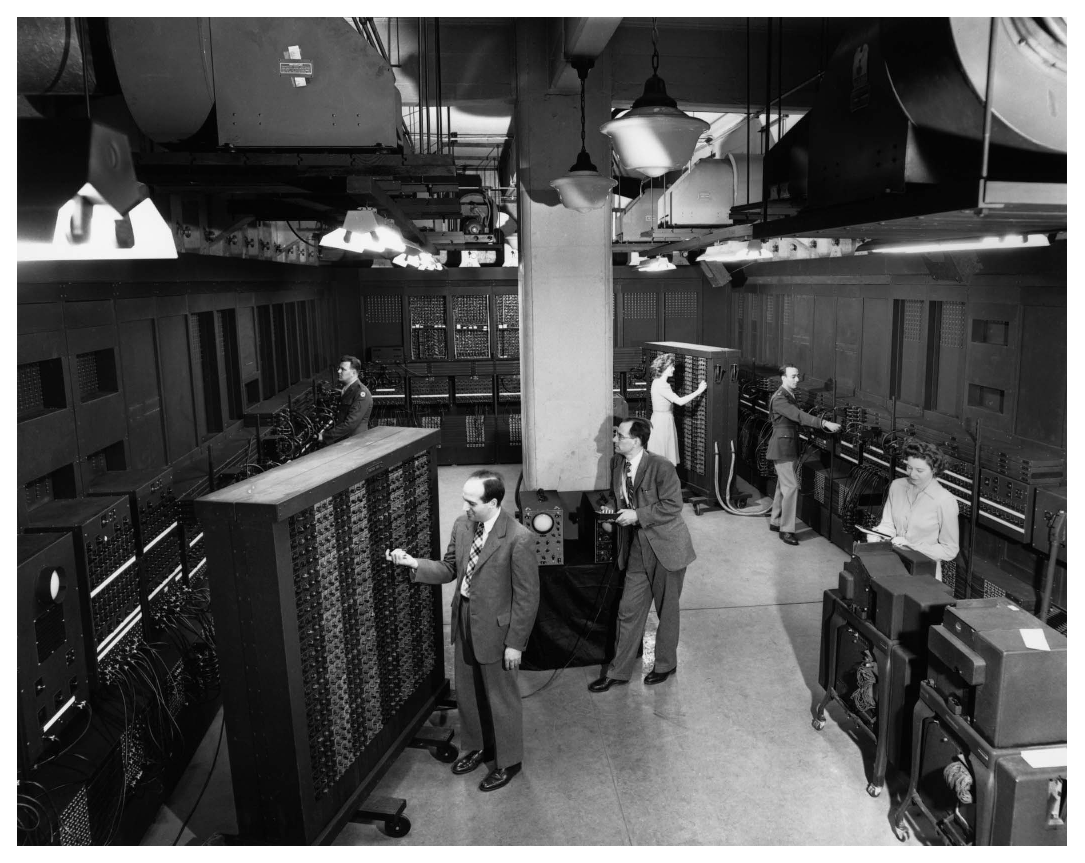
\includegraphics[width=\columnwidth]{figures/eniac1946.eps}
    }
    {
      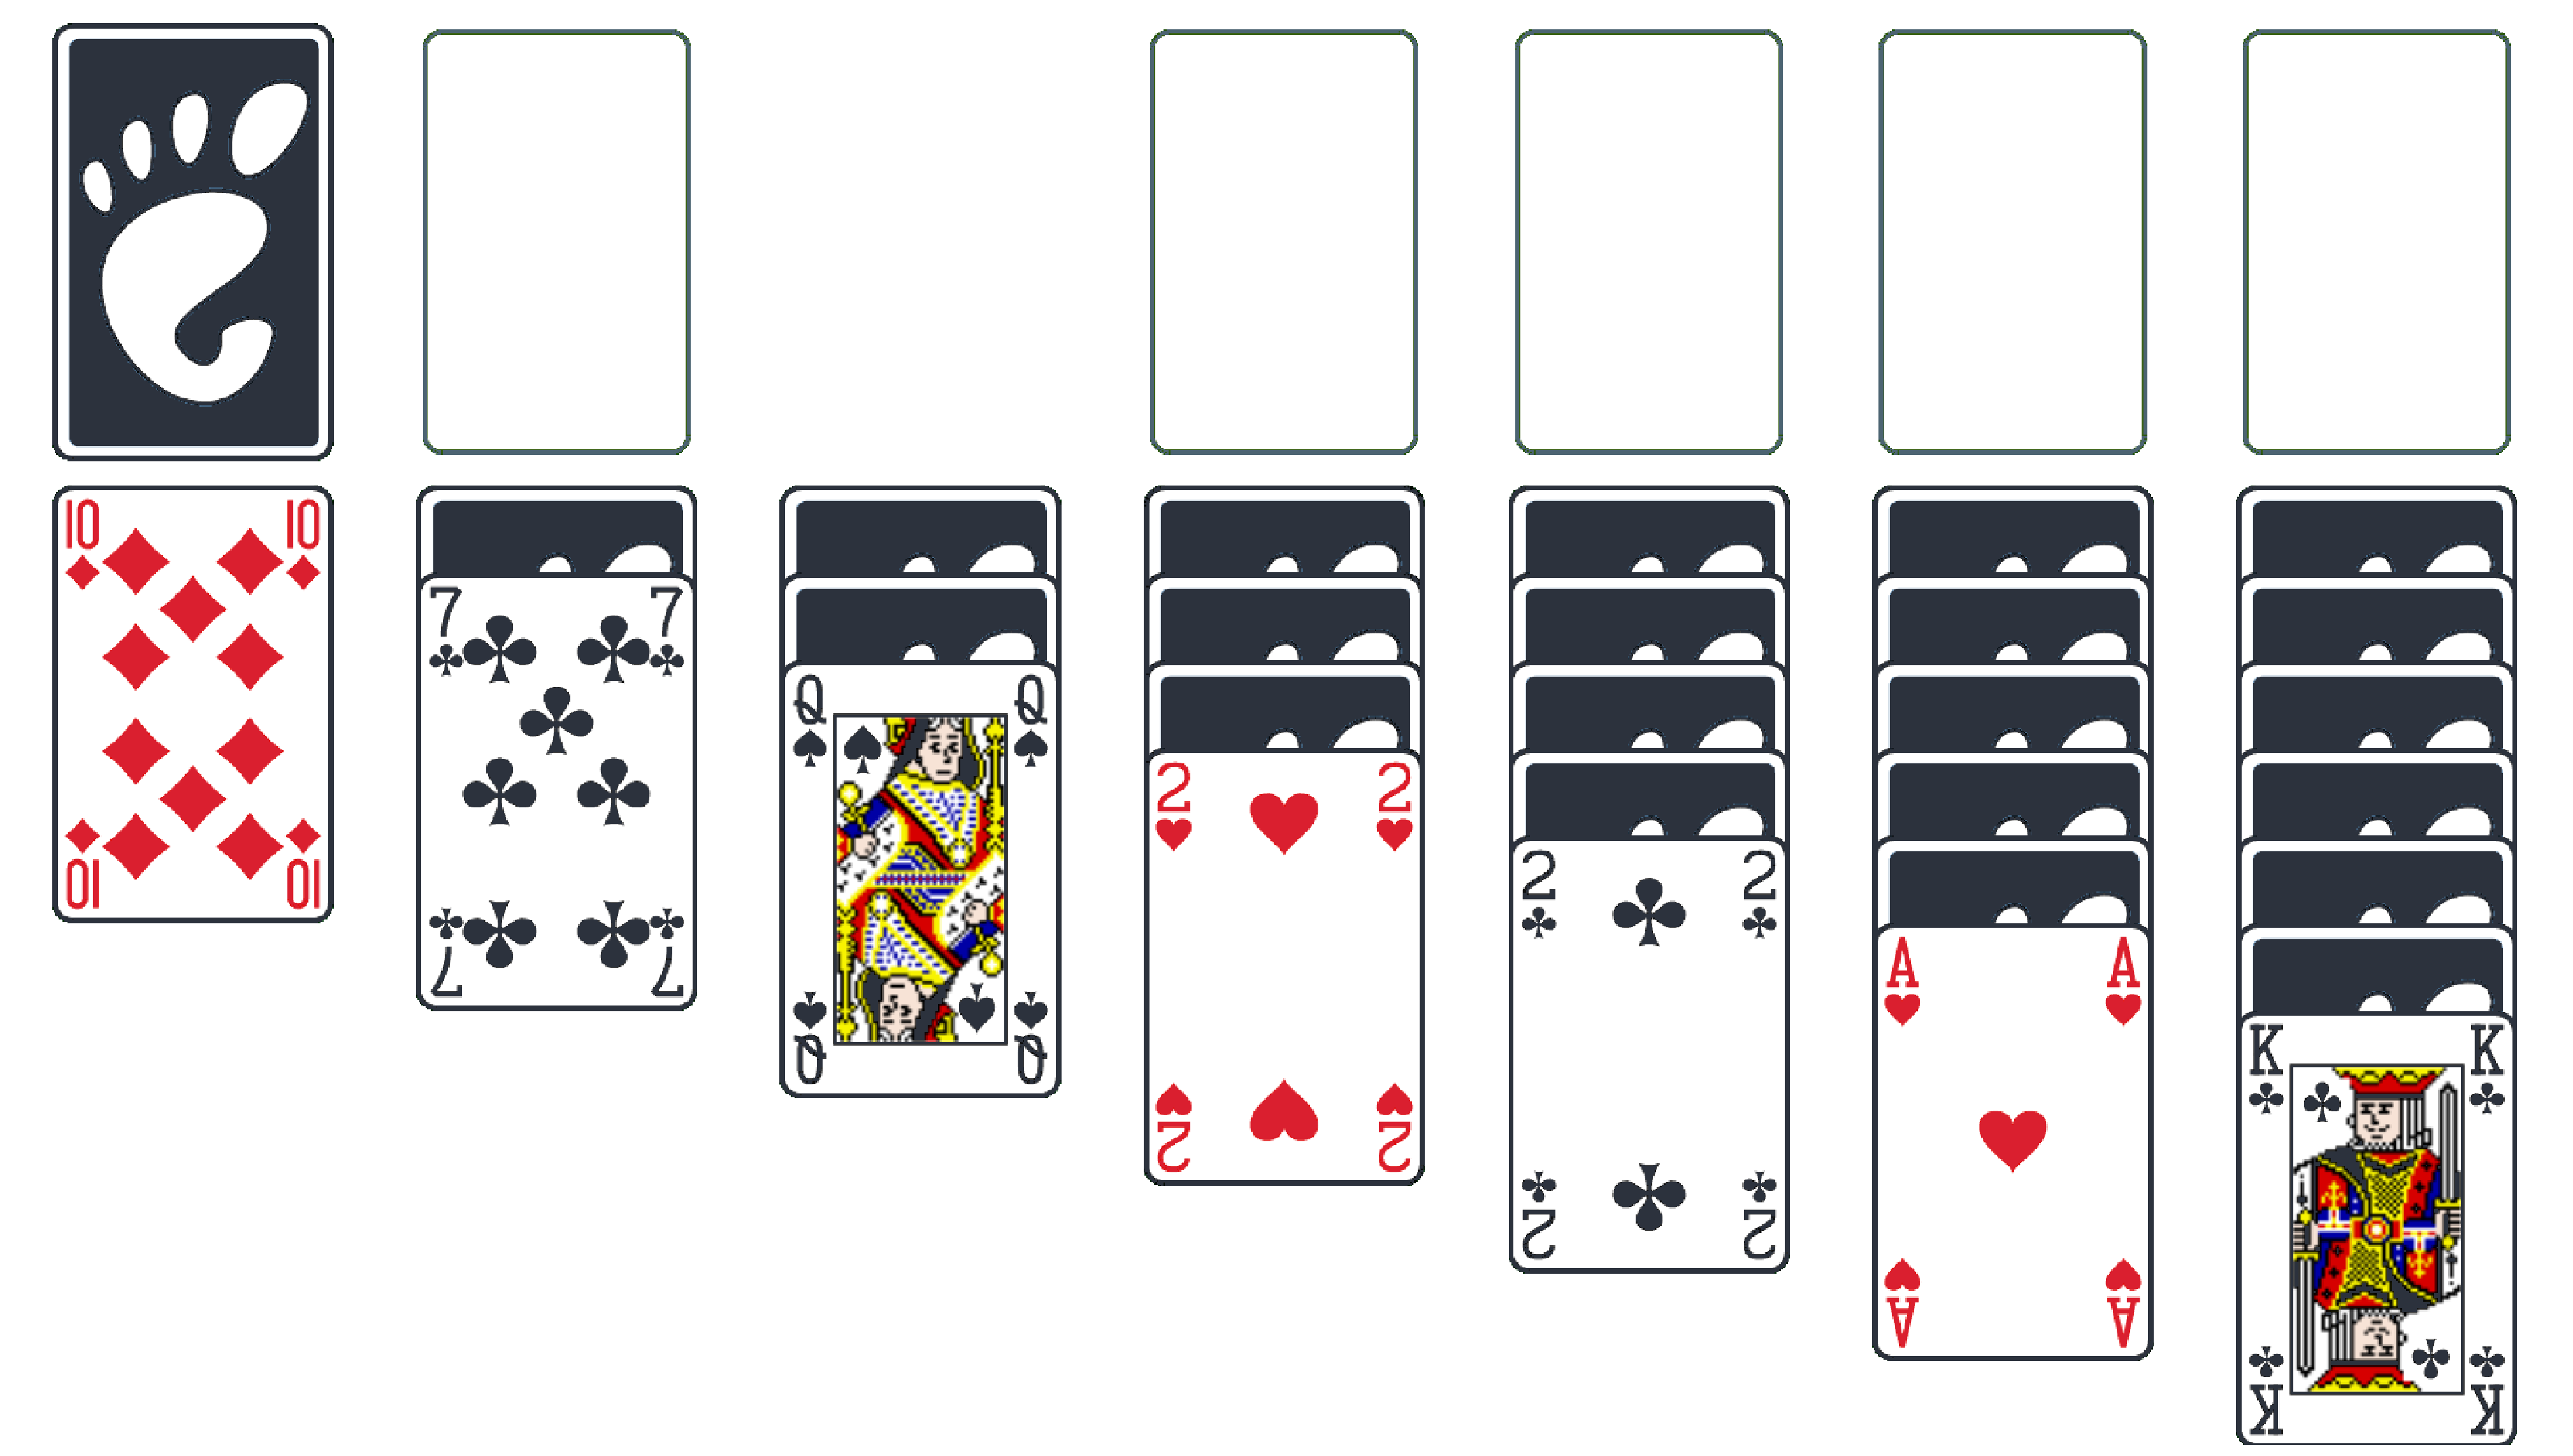
\includegraphics[width=\columnwidth]{figures/solitaire.eps}
      \begin{itemize}
	\item What is a probability of success in solitaire?
	\begin{itemize}
	  \item Too complex for an analytical calculations
	  \item Lets try $N = 100$ times and count wins
	  \item With $N \rightarrow \infty$ we are getting closer to correct result
	\end{itemize}
      \end{itemize}
    }
 
\vfill\null
\end{wideslide}

\begin{wideslide}[toc = Simple Monte Carlo, method=direct]{Simple Monte Carlo - coin flipping}
\null\vfill

  \begin{itemize}
    \item What is the probability of getting head / tail when throwing a coin?
  \end{itemize}
  
  \begin{minipage}{0.7\textwidth}
  \begin{itemize}
    \item One can use MC method to calculate this:
    \begin{itemize}
      \item get $N$ times a random number $x \in [0,1)$
      \item check how many ($n$) times $x < 0.5$
      \item $P = \frac{n}{N}$
    \end{itemize}
    \item One-line example in Python:
  \end{itemize}
  \end{minipage}\begin{minipage}{0.3\textwidth}
		  
\includegraphics[width=0.5\columnwidth]{figures/coin.eps}
                \end{minipage}

  {\small\color{pdcolor3}
  \begin{verbatim}
MC = lambda N: len(filter(lambda x: random.random() < 0.5, range(N))) / float(N)     
  \end{verbatim}
  }
  \begin{minipage}{0.55\textwidth}
  \begin{itemize}
   \item If you do not like one-liners:
  \end{itemize}
  \vspace{-20pt}  
  {\small\color{pdcolor3}
  \begin{verbatim}
def MonteCarlo(N):
  n = 0
  for _ in range(N):
    if (random.random() < 0.5): n += 1
  return float(n) / N   
  \end{verbatim}
  }
  \end{minipage}\begin{minipage}{0.45\textwidth}
		  \vspace{-10pt}
		  \begin{itemize}
		   \item Some results for MC(100):
		   \item[]
		   0.51, 0.48, 0.61, 0.46, 0.57, 0.46
		   \item Some results for MC(100000):
		   \item[]
		   0.50139, 0.49798, 0.49933, 0.5005
		  \end{itemize}
                \end{minipage}

\vfill\null
\end{wideslide}

\begin{slide}[toc=PRNG]{Pseudorandom number generator}
\null\vfill

  \begin{itemize}
    \item PRNG is an algorithm for generating a sequence of ``random'' numbers
    \item Example: middle-square method (used in ENIAC)
    \begin{itemize}
      \item take $n$-digit number as your seed
      \item square it to get $2n$-digit number (add leading zeroes if necessary)
      \item $n$ middle digits are the result and the seed for next number
    \end{itemize}
    \item Middle-square method for $n = 4$ and base seed = $1111$:
  \end{itemize}
  \vspace{-10pt}
  \begin{eqnarray*}
    1111^2 & = & {\color{pdcolor3}01}2343{\color{pdcolor3}21} \rightarrow 2343 \\
    2343^2 & = & {\color{pdcolor3}05}4896{\color{pdcolor3}49} \rightarrow 4896 \\
    & \vdots & \\
    1111^2 & = & {\color{pdcolor3}01}2343{\color{pdcolor3}21} \rightarrow 2343 
  \end{eqnarray*}
    
\vfill\null
\end{slide}

\begin{slide}[toc=]{Pseudorandom number generator}
\null\vfill

  \begin{itemize}
    \item Nowadays, more sophisticated PRNGs exist, but they also suffer on some common problems:
    \begin{itemize}
      \item periodicity / different periodicity for different base seed
      \item nonuniformity of number distributions
      \item correlation of successive numbers
    \end{itemize}
  \end{itemize}

  \twocolumn
  {
    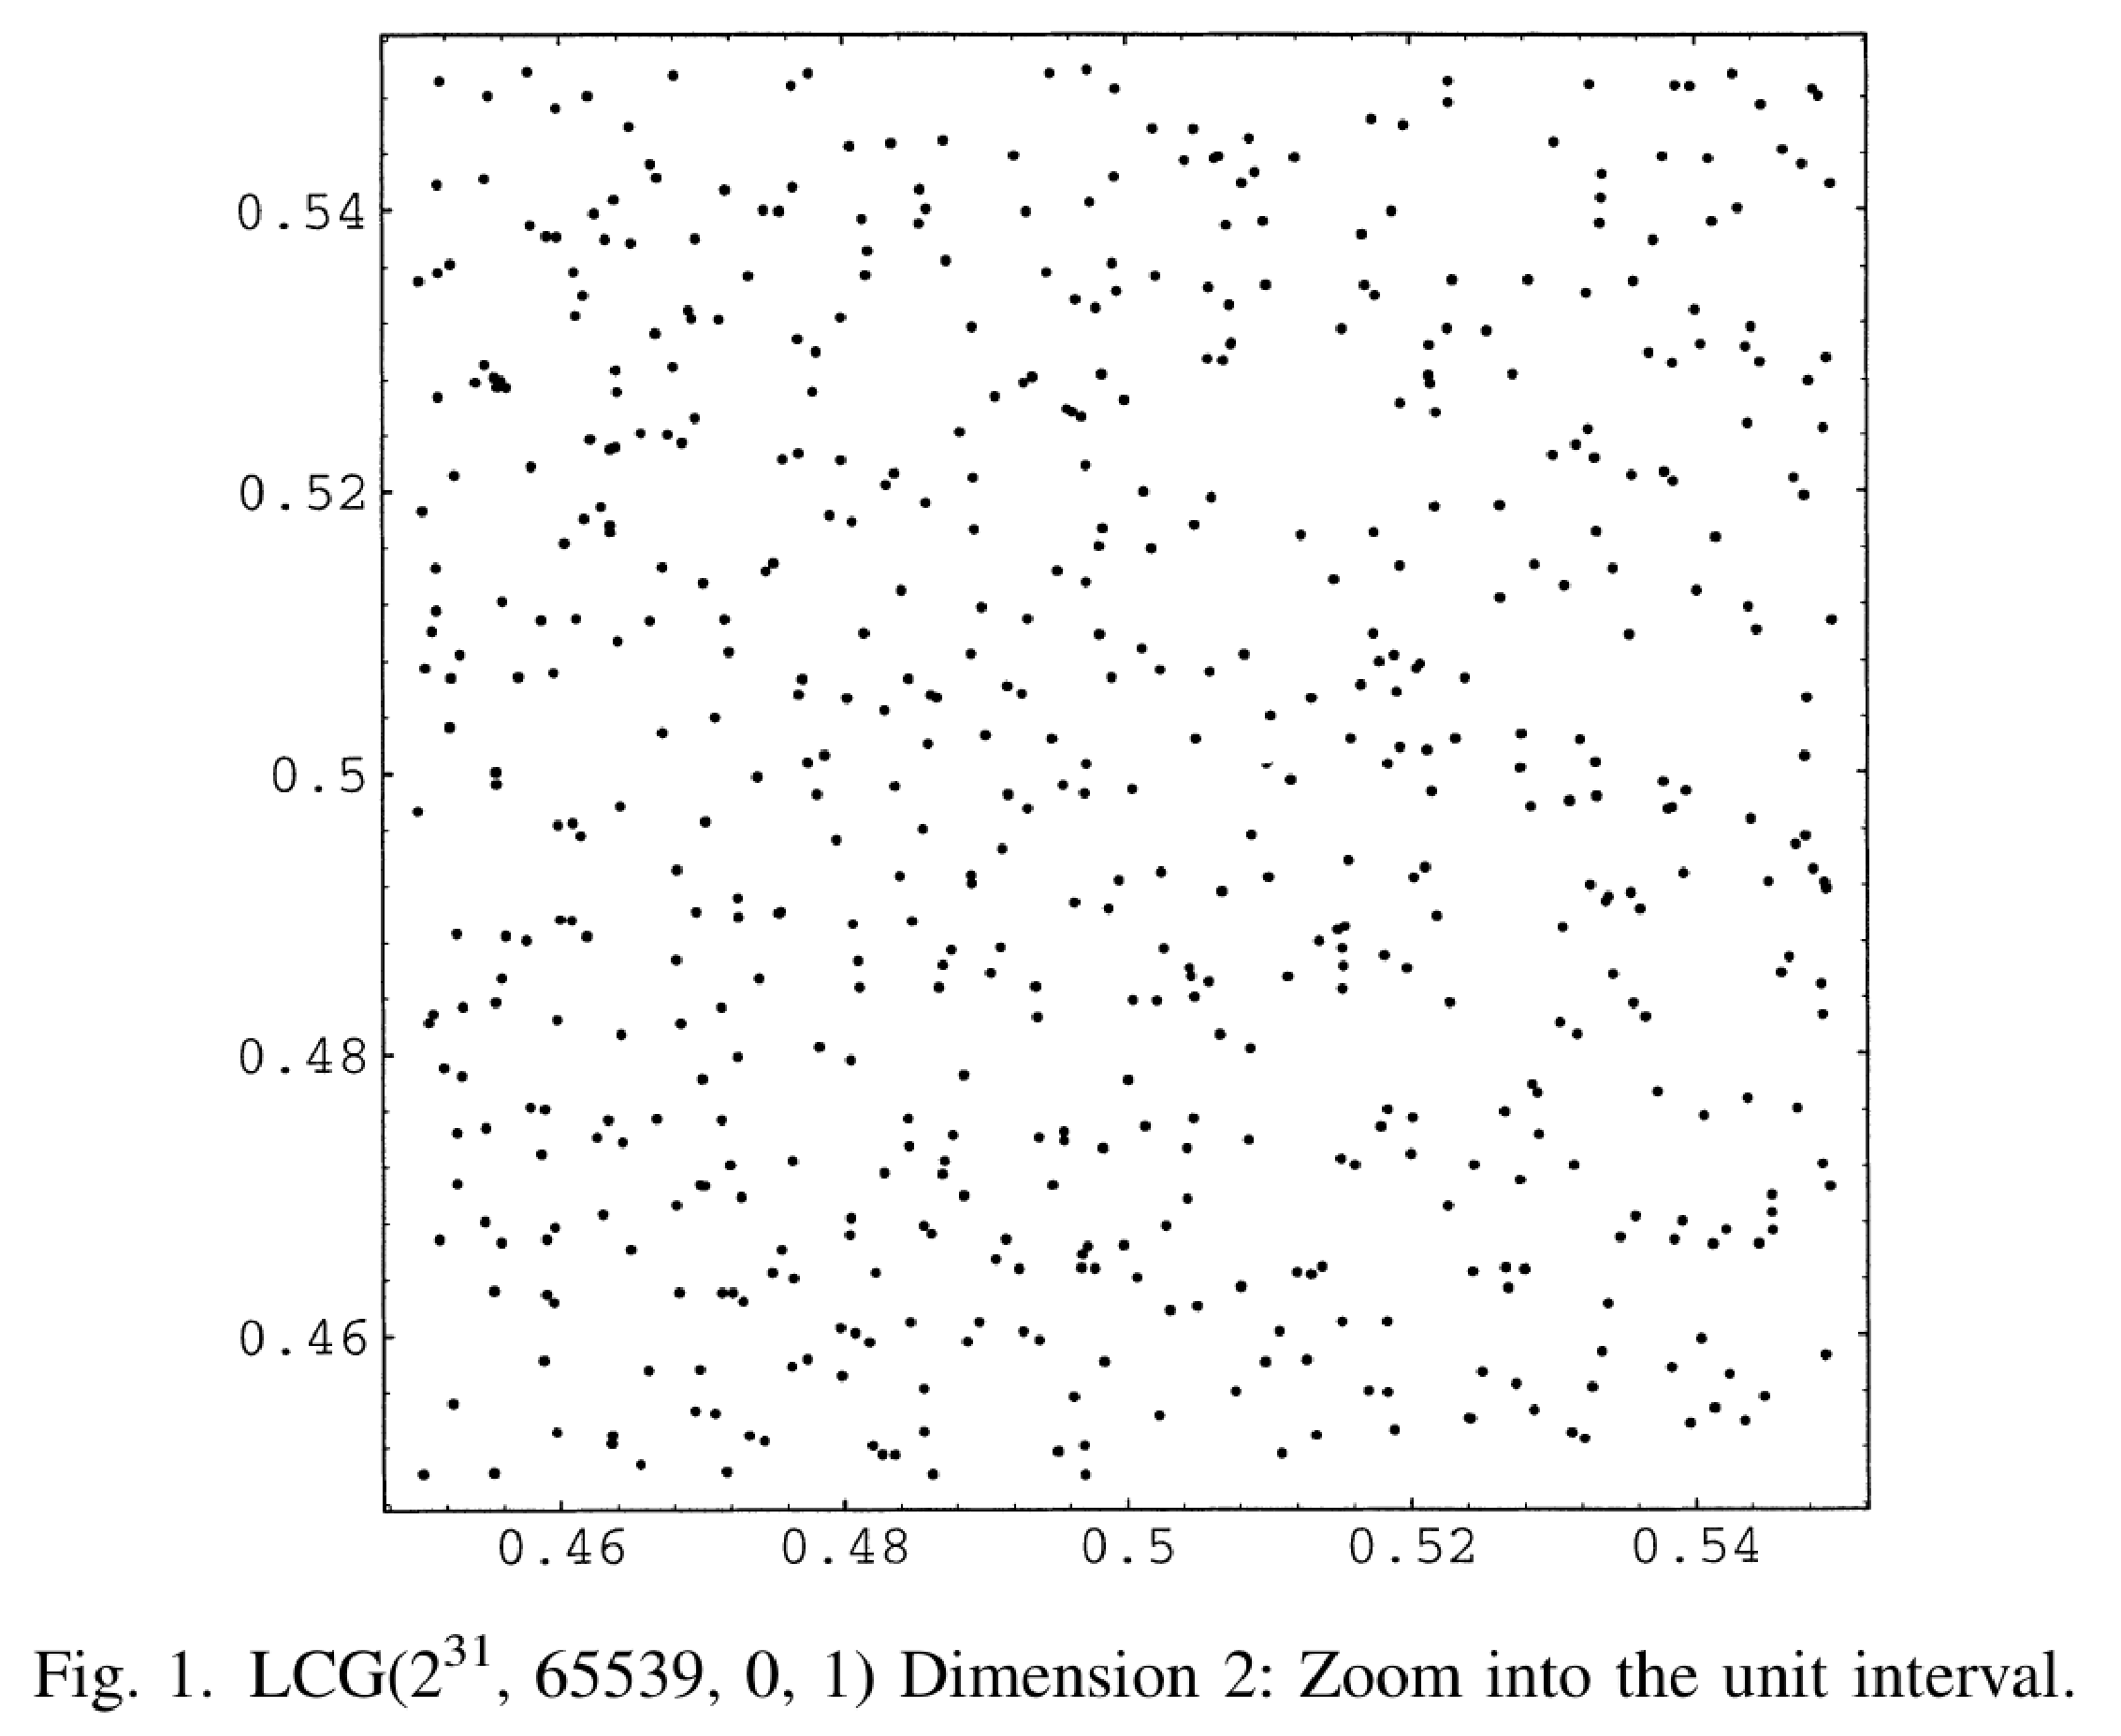
\includegraphics[width=\columnwidth]{figures/random2d.eps}
  }
  {
    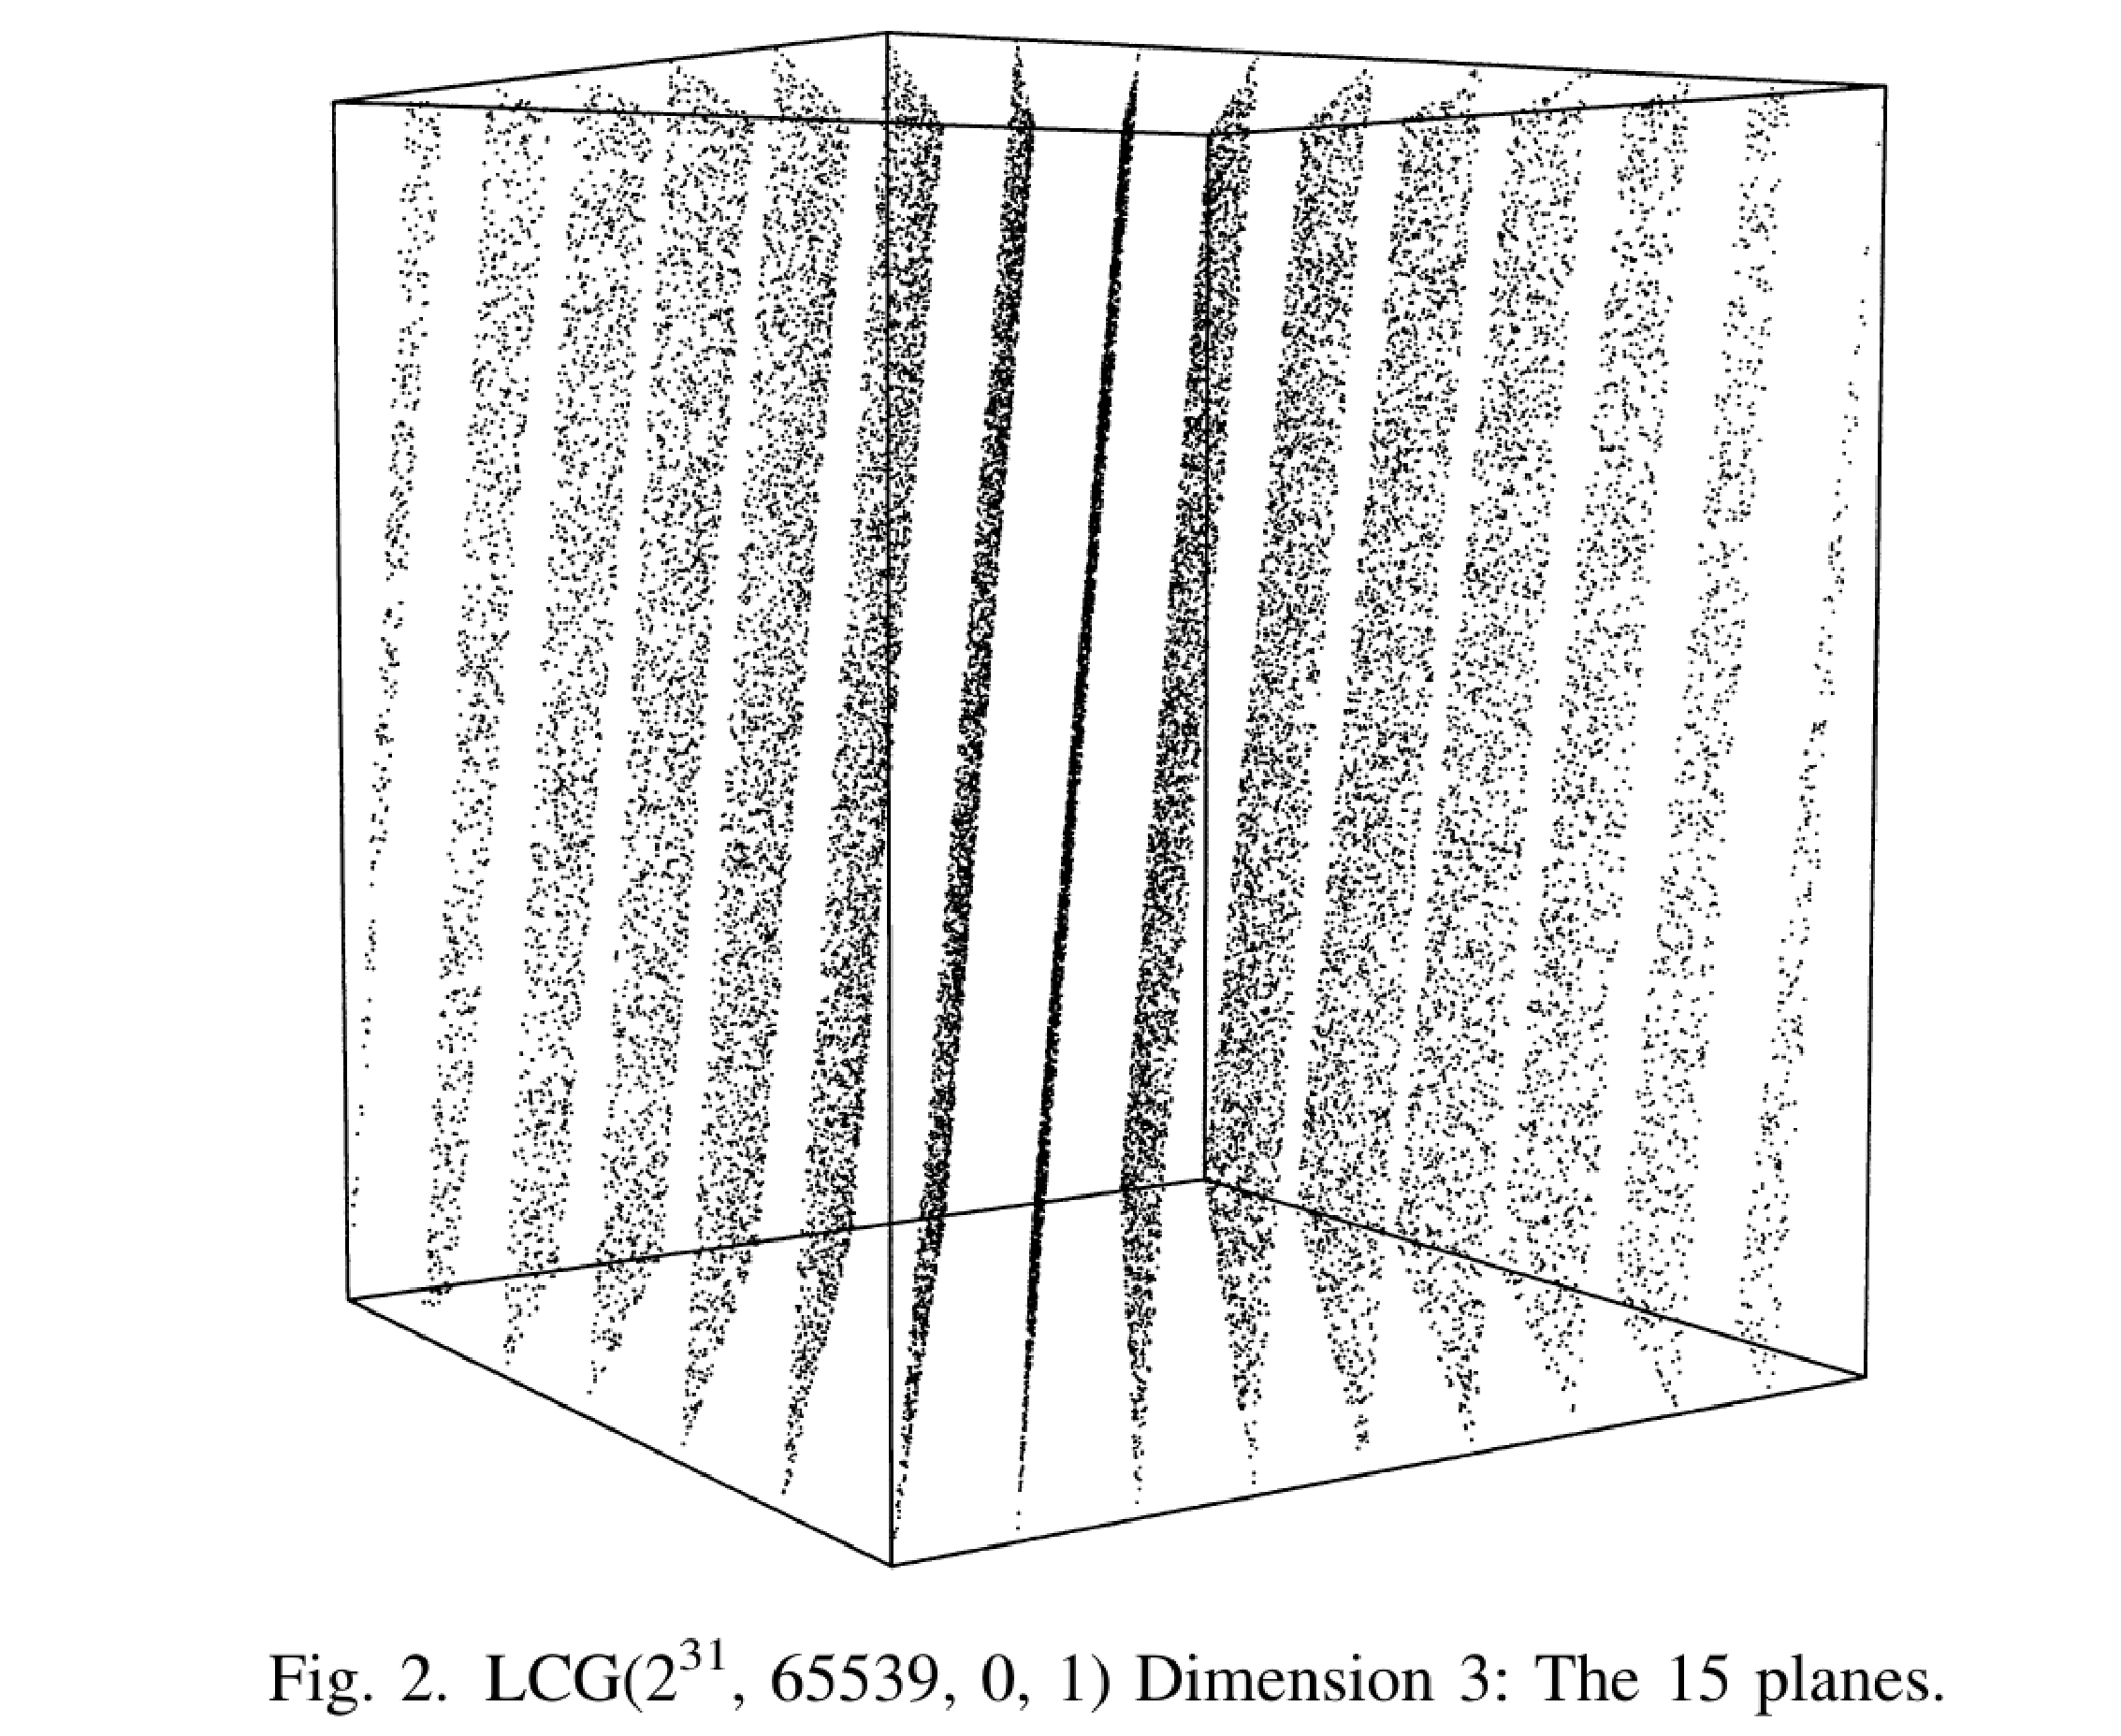
\includegraphics[width=\columnwidth]{figures/random3d.eps}
  }
  {\it\color{pdcolor3}Mathematics and Computers in Simulations 46 (1998) 485-505}
\vfill\null
\end{slide}

\begin{slide}[toc=Hit-or-Miss method]{MC integration (Hit-or-Miss method)}
\null\vfill

  Lets do the following integration using MC method:
  
  $$\int_0^1 f(x)dx = \int_0^1 \left(\frac{1}{2}x\right) dx = \left.\frac{1}{2}\frac{x^2}{2}\right|_{0}^{1} = \frac{1}{4}$$

  \twocolumn
  {
    \sep
    \begin{itemize}
     \item take a random point from the $[0,1]\times[0,1]$ square
     \item compare it to your $f(x)$
     \item repeat $N$ times
     \item count $n$ points below the function
     \item you results is given by
     $$\int_0^1 f(x)dx = P_{\square} \cdot \frac{n}{N} = \frac{n}{N}$$
    \end{itemize}
  }
  {
    \usetikzlibrary{calc}

\begin{tikzpicture}

  \draw[>=latex, <->, thick] node[left, yshift = 4cm]{$y$} ++ (0, 4) -- (0, 0) -- node[below, xshift = 2cm]{$x$} ++ (4,0);
  
  \foreach \x in {1,...,200}
  {
    \pgfmathparse{rnd}
    \pgfmathsetmacro{\a}{2.9*\pgfmathresult + 0.05}
    \pgfmathparse{rnd}
    \pgfmathsetmacro{\b}{2.9*\pgfmathresult + 0.05}
    \pgfmathsetmacro{\c}{\a - 2.0 * \b}
        
    \ifthenelse{\lengthtest{\c pt > 0.2 pt}}{\draw[filled, color=pdcolor7] (\a, \b) circle (0.03);}{}
    \ifthenelse{\lengthtest{\c pt < - 0.2 pt}}{\draw[filled, color=pdcolor6] (\a, \b) circle (0.03);}{}
  }

  \draw[ultra thick] (0,0) -- node[yshift = 1.5cm, xshift = 2cm]{$f(x) = \frac{1}{2}x$} ++ (4,2);
  
  \draw[color=pdcolor3, dashed] node[left, yshift = 3cm]{1} ++ (0, 3) -- (3,3) -- node[yshift = -1.75cm]{1} (3, 0);
      
\end{tikzpicture}

  }
  
\vfill\null
\end{slide}

\begin{emptyslide}{MC integration results}
\null\vfill

  \twocolumn
  {
    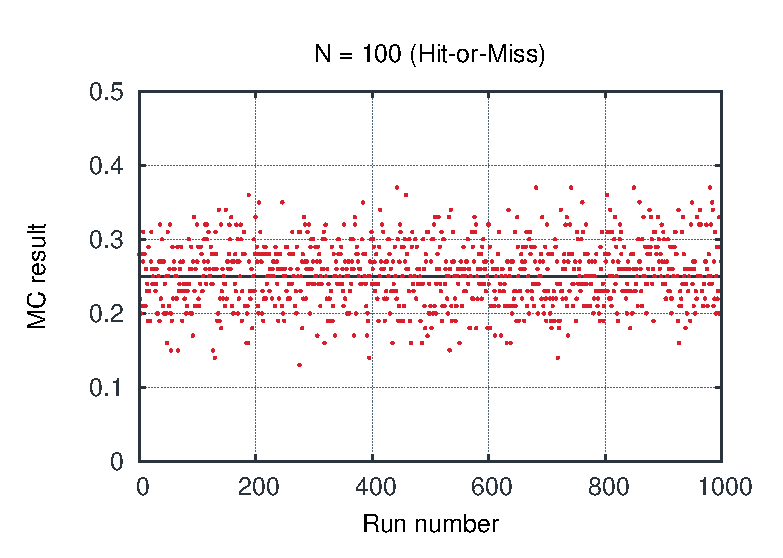
\includegraphics[width=\columnwidth]{figures/int100.eps}
    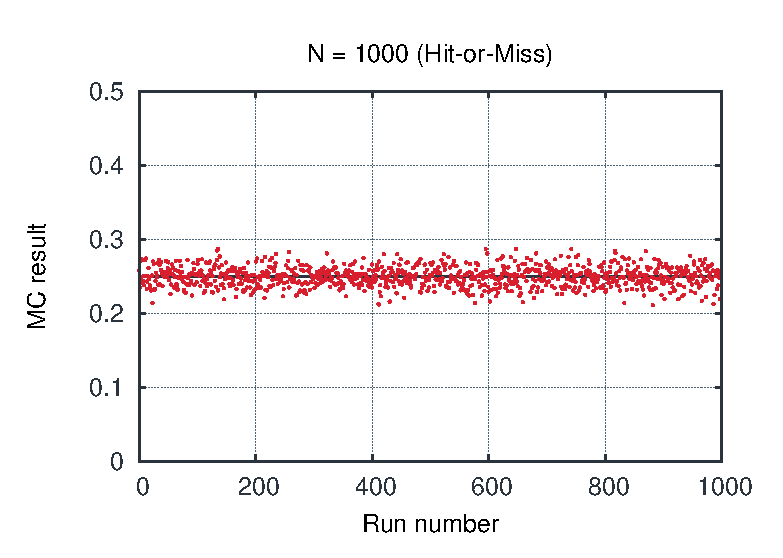
\includegraphics[width=\columnwidth]{figures/int1000.eps}
  }
  {
    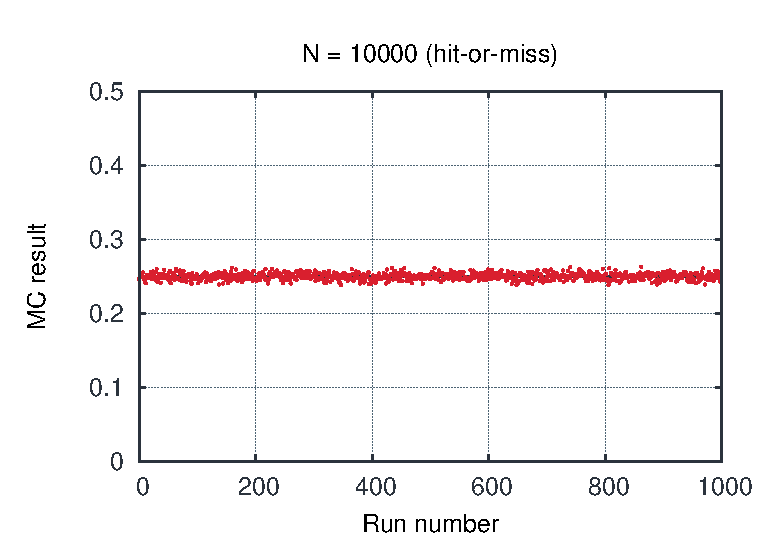
\includegraphics[width=\columnwidth]{figures/int10000.eps}
    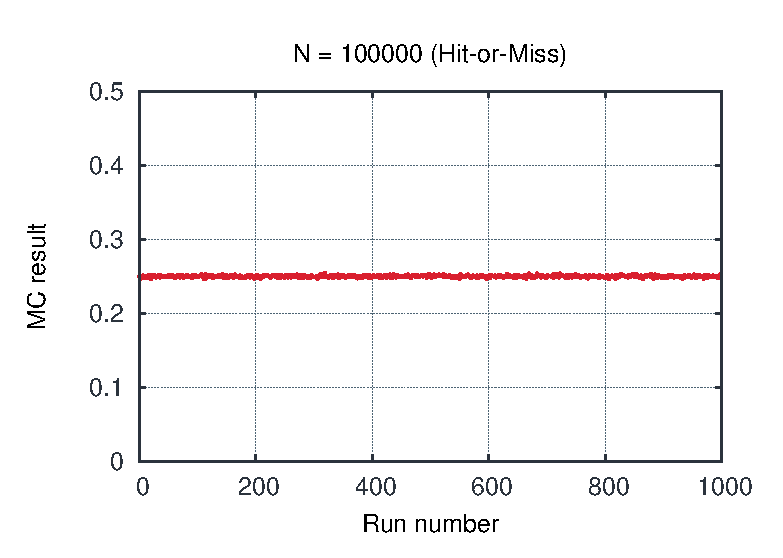
\includegraphics[width=\columnwidth]{figures/int100000.eps}
  }

\vfill\null
\end{emptyslide}


\begin{slide}{Optimization of MC}
\null\vfill

  \twocolumn
  {
    \scalebox{.75}{\usetikzlibrary{calc}

\begin{tikzpicture}

  \draw[>=latex, <->, thick] node[left, yshift = 4cm]{$y$} ++ (0, 4) -- (0, 0) -- node[below, xshift = 2cm]{$x$} ++ (4,0);
  
  \foreach \x in {1,...,200}
  {
    \pgfmathparse{rnd}
    \pgfmathsetmacro{\a}{2.9*\pgfmathresult + 0.05}
    \pgfmathparse{rnd}
    \pgfmathsetmacro{\b}{2.9*\pgfmathresult + 0.05}
    \pgfmathsetmacro{\c}{\a - 2.0 * \b}
        
    \ifthenelse{\lengthtest{\c pt > 0.2 pt}}{\draw[filled, color=pdcolor7] (\a, \b) circle (0.03);}{}
    \ifthenelse{\lengthtest{\c pt < - 0.2 pt}}{\draw[filled, color=pdcolor6] (\a, \b) circle (0.03);}{}
  }

  \draw[ultra thick] (0,0) -- node[yshift = 1.5cm, xshift = 2cm]{$f(x) = \frac{1}{2}x$} ++ (4,2);
  
  \draw[color=pdcolor3, dashed] node[left, yshift = 3cm]{1} ++ (0, 3) -- (3,3) -- node[yshift = -1.75cm]{1} (3, 0);
      
\end{tikzpicture}
}
  }
  {
    \scalebox{.75}{\usetikzlibrary{calc}

\begin{tikzpicture}

  \draw[>=latex, <->, thick] node[left, yshift = 4cm]{$y$} ++ (0, 4) -- (0, 0) -- node[below, xshift = 2cm]{$x$} ++ (4,0);
  
  \foreach \x in {1,...,200}
  {
    \pgfmathparse{rnd}
    \pgfmathsetmacro{\a}{2.9*\pgfmathresult + 0.05}
    \pgfmathparse{rnd}
    \pgfmathsetmacro{\b}{1.4*\pgfmathresult + 0.05}
    \pgfmathsetmacro{\c}{\a - 2.0 * \b}
        
    \ifthenelse{\lengthtest{\c pt > 0.2 pt}}{\draw[filled, color=pdcolor7] (\a, \b) circle (0.03);}{}
    \ifthenelse{\lengthtest{\c pt < - 0.2 pt}}{\draw[filled, color=pdcolor6] (\a, \b) circle (0.03);}{}
  }

  \draw[ultra thick] (0,0) -- node[yshift = 1.5cm, xshift = 2cm]{$f(x) = \frac{1}{2}x$} ++ (4,2);
  
  \draw[color=pdcolor3, dashed] node[left, yshift = 1.5cm]{0.5} ++ (0, 1.5) -- (3,1.5) -- node[yshift = -1.75cm]{1} (3, 0);
      
\end{tikzpicture}
}
  }

  \begin{itemize}
   \item You want to avoid drawing ``red'' points as they do not contribute to your integral
   \item You can choose any rectangle as far as it contains maximum of $f(x)$ in given range
  \end{itemize}

\vfill\null
\end{slide}

\begin{slide}[toc=]{Optimization of MC}
\null\vfill

  \twocolumn
  {
    \begin{itemize}
      \item Lets consider the following function:
  
      $$F(Q^2) = \frac{1}{(1 + Q^2)^2}$$
      {\it\color{pdcolor3} more or less dipole form factor}
      
      \item Integrating this function over $Q^2$ is highly inefficient
      
      \item However, one can integrate by substitution to get better performance, e.g.
      
      $$x = \mbox{log}_{10}(Q^2)$$
      
    \sep{\it\color{pdcolor6}don't forget about Jacobian}

    \end{itemize}

  }
  {
    \usetikzlibrary{calc}

\pgfplotsset{every  tick/.style={pdcolor3,}, minor x tick num=1,}

\begin{tikzpicture}

  \begin{axis}[xlabel = $Q^2$, ylabel = $F(Q^2)$, ylabel near ticks, domain=1:10, scale=0.5, axis lines = left, inner axis line style={>=latex}, ymin = 0, ymax = 0.275, xmin = 1, xmax = 10.5]
    
    \addplot[mark=none, color=pdcolor1, ultra thick] {1 / (1 + x) / (1 + x)};
    \addplot[mark=none, dashed, color=pdcolor3, thick] coordinates {(1,0.25) (10,0.25) (10,0)};

    
    \foreach \x in {1,...,200}
    {
      \pgfmathparse{rnd}
      \pgfmathsetmacro{\a}{9.0*\pgfmathresult + 0.95}
      \pgfmathparse{rnd}
      \pgfmathsetmacro{\b}{0.23*\pgfmathresult + 0.01}
      \pgfmathsetmacro{\c}{\b - 1 / (1 + \a) / (1 + \a)}
      	  
      \ifthenelse{\lengthtest{\c pt > 0.01 pt}}{\addplot[mark=*, mark size = 1pt, color=pdcolor6] coordinates {(\a, \b)};}{}
      \ifthenelse{\lengthtest{\c pt < -0.01 pt}}{\addplot[mark=*, mark size = 1pt, color=pdcolor7] coordinates {(\a, \b)};}{}
    }
    
  \end{axis}

\end{tikzpicture}
    \vspace{-10pt}
    \usetikzlibrary{calc}

\pgfplotsset{every  tick/.style={pdcolor3,}, minor x tick num=1,}

\begin{tikzpicture}

  \begin{axis}[xlabel = {$x = \mbox{log}_{10}(Q^2)$}, ylabel = $F(x)$, ylabel near ticks, domain=-2:1, scale=0.5, axis lines = left, inner axis line style={>=latex}, ymin = 0, ymax = 1.25, xmin = -2, xmax = 1.25]
    
    \addplot[mark=none, color=pdcolor1, ultra thick] {1 / (1 + 10^x) / (1 + 10^x)};
    \addplot[mark=none, dashed, color=pdcolor3, thick] coordinates {(-2,1) (1,1) (1,0)};
    
    \foreach \x in {1,...,200}
    {
      \pgfmathparse{rnd}
      \pgfmathsetmacro{\a}{-2.90*\pgfmathresult + 0.95}
      \pgfmathparse{rnd}
      \pgfmathsetmacro{\b}{0.90*\pgfmathresult + 0.05}
      \pgfmathsetmacro{\d}{-0.175 * (\a + 2) * (\a + 2) + 1}
      \pgfmathsetmacro{\c}{\b - \d}
      	  
      \ifthenelse{\lengthtest{\c pt > 0.1 pt}}{\addplot[mark=*, mark size = 1pt, color=pdcolor6] coordinates {(\a, \b)};}{}
      \ifthenelse{\lengthtest{\c pt < - 0.1 pt}}{\addplot[mark=*, mark size = 1pt, color=pdcolor7] coordinates {(\a, \b)};}{}
    }
    
  \end{axis}

\end{tikzpicture}
    
  }
    
\vfill\null
\end{slide}

\begin{slide}[toc=Crude method]{MC integration (Crude method)}
\null\vfill

  Lets do the following integration using MC method once again:
  
  $$\int_0^1 f(x)dx = \int_0^1 \left(\frac{1}{2}x\right) dx = \left.\frac{1}{2}\frac{x^2}{2}\right|_{0}^{1} = \frac{1}{4}$$
  \twocolumn
  {
    \begin{itemize}
      \item One can approximate integral
      \vspace{-5pt}
      $$\int_a^b f(x) dx \approx \frac{b - a}{N}\sum_{i=1}^{N} f(x_i)$$
     
      where $x_i$ is a random number from $[a, b]$
      
      \item It can be shown that Crude method is more accurate than Hit-or-Miss
      
      \item We will skip the math and look at some comparisons
      
    \end{itemize}
  }
  {
    \usetikzlibrary{calc}

\begin{tikzpicture}

  \draw[>=latex, <->, thick] node[left, yshift = 4cm]{$y$} ++ (0, 4) -- (0, 0) -- node[below, xshift = 2cm]{$x$} ++ (4,0);
  
  \foreach \x in {1,...,14}
  {
    \pgfmathparse{rnd}

    \pgfmathsetmacro{\a}{0.2 * \x + 0.05 + 0.1 * \pgfmathresult - 0.05}
        
    \draw[filled, color=pdcolor7] (\a, 0) circle (0.03);
    
    \draw[thin, color=pdcolor3, dashed] (\a, 0) -- (\a, 0.5*\a);
  }

  \draw[ultra thick] (0,0) -- node[yshift = 1.5cm, xshift = 2cm]{$f(x) = \frac{1}{2}x$} ++ (4,2);
        
\end{tikzpicture}

  }

\vfill\null
\end{slide}

\begin{emptyslide}{Methods comparison}
\null\vfill

  \twocolumn
  {
    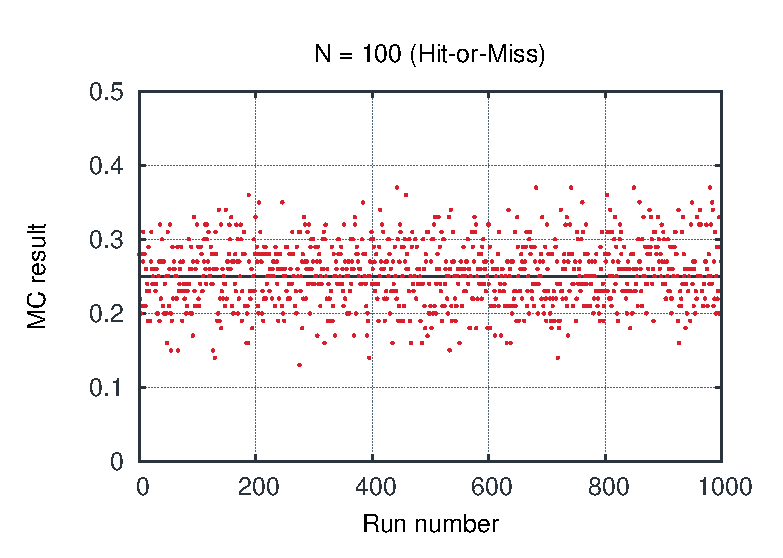
\includegraphics[width=\columnwidth]{figures/int100.eps}
    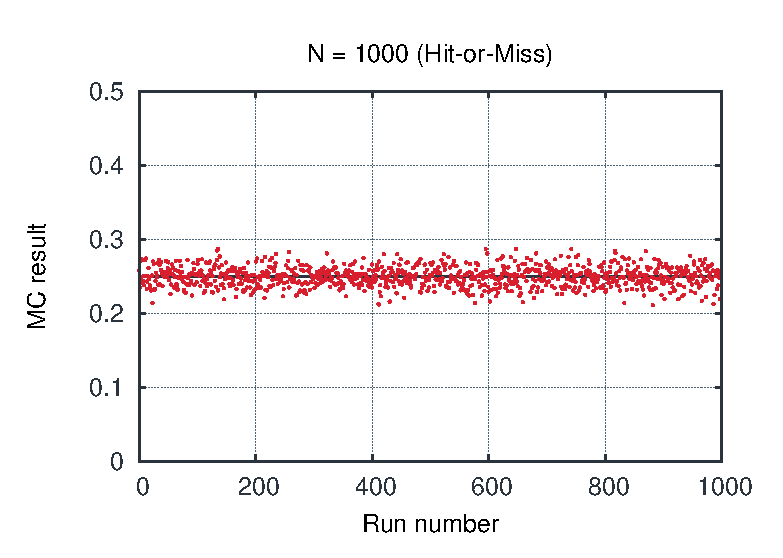
\includegraphics[width=\columnwidth]{figures/int1000.eps}
  }
  {
    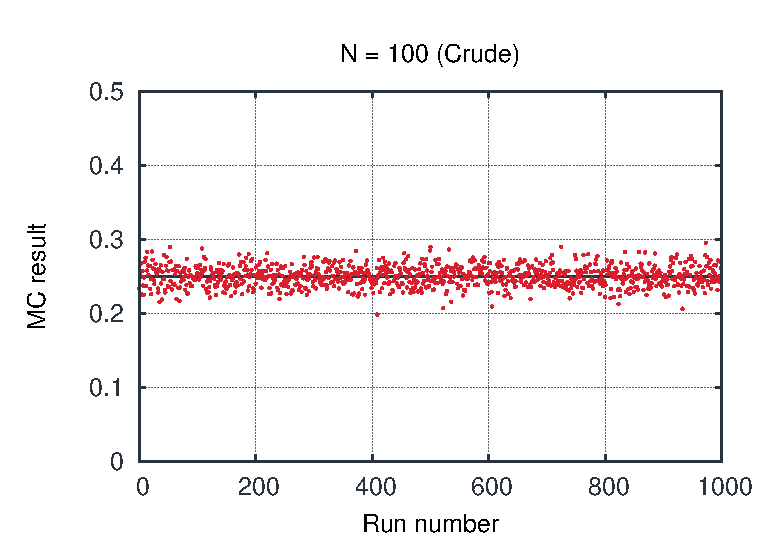
\includegraphics[width=\columnwidth]{figures/int2100.eps}
    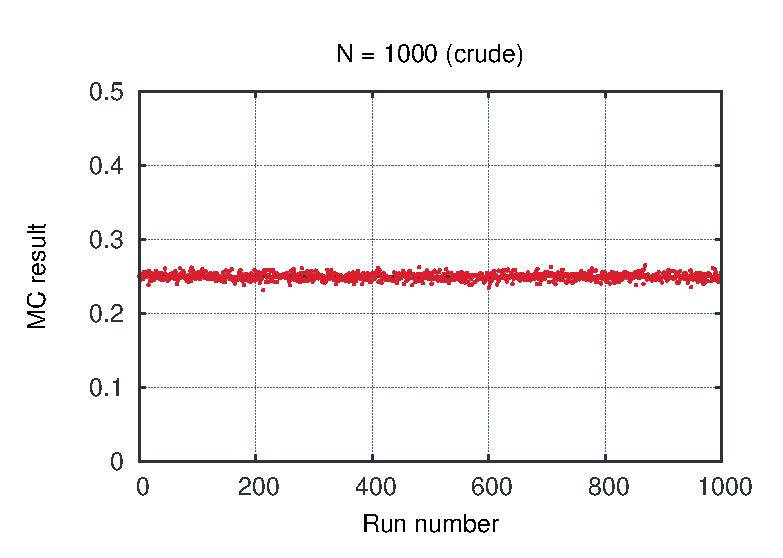
\includegraphics[width=\columnwidth]{figures/int21000.eps}
  }

\vfill\null
\end{emptyslide}



\section[toc=Quasi-elastic scattering]{Quasi-elastic scattering \\ \small{Building a generator step by step}}

\begin{wideslide}[toc=QEL on free N]{Quasi-elastic scattering on a free nucleon}
\null\vfill

  \myBox{Llewellyn-Smith formula}
  
  $$\frac{d\sigma}{d|q^2|} {{\nu_l + n \rightarrow l^- + p}\choose{\bar\nu_l + p \rightarrow l^+ + n}} = \frac{M^2G_F^2\cos\theta_C}{8\pi E_\nu^2}\left[A(q^2) \mp B(q^2)\frac{(s - u)}{M^2} + C(q^2)\frac{(s - u)^2}{M^4}\right]$$
  
  \myBox{Notation}
  
  \begin{itemize}
    \item Constants: $M$ - nucleon mass, $G_F$ - Fermi constant, $\theta_C$ - Cabibbo angle,
    \item $q^2 = (k - k')^2 = (p' - p)^2$ - four-momentum squared, where $k$, $k'$, $p$, $p'$ are four-momenta of initial and final lepton, initial and final nucleon
    \item $E_\nu$ - neutrino energy
    \item $s = (k + k')^2$ and $u = (k - p')^2$ - Mandelstam variables
  \end{itemize}

  
\vfill\null
\end{wideslide}

\begin{wideslide}[toc=]{Quasi-elastic scattering on a free nucleon}
\null\vfill

  \myBox{Llewellyn-Smith formula}
  
  $$\frac{d\sigma}{d|q^2|} {{\nu_l + n \rightarrow l^- + p}\choose{\bar\nu_l + p \rightarrow l^+ + n}} = \frac{M^2G_F^2\cos\theta_C}{8\pi E_\nu^2}\left[A(q^2) \mp B(q^2)\frac{(s - u)}{M^2} + C(q^2)\frac{(s - u)^2}{M^4}\right]$$
  
  \myBox{General idea}
  
  \begin{itemize}
    \item Having $k$ and $p$, generate $k'$ and $p'$
    \item Calculate $q^2$ and $(s - u) = 4ME_\nu + q^2 -m^2$ based on generated kinematics
    \item Calculate cross section
    \item Repeat $N$ times and the result is given by: 
    
    $$\sigma_{total} \sim \frac{1}{N} \sum\limits_{i = 1}^N \sigma (q_i^2)$$
    
  \end{itemize}

\vfill\null
\end{wideslide}

\begin{slide}{Generating kinematics}
\null\vfill

  \twocolumn
{
\centering
\begin{tikzpicture}

  \draw [notFilled=pdcolor3, thin] (-0.5, -0.5) -- (-0.5, 1.5) -- node[below, yshift = -0.25 cm] {\color{pdcolor1}LAB} (3.5, 1.5) -- (3.5, -0.5) -- (-0.5, -0.5);

  \draw [filled = pdcolor1] (0, 0) circle (0.25);
  \draw [filled = pdcolor6] (3, 0) circle (0.25);
  \draw [line, ultra thick, ->] (0.25, 0) -- node[above] {$\vec p_\nu$} (1.5, 0);
  \draw [line, ultra thick, ->, color = pdcolor6] (2.75, 0.1) -- node[above, xshift = 0.25cm] {$\vec p_N$} (2.0, 0.5);

\end{tikzpicture}
}
{
\centering
\begin{tikzpicture}

  \draw [notFilled=pdcolor3, thin] (-0.5, -0.5) -- (-0.5, 1.5) -- node[below, yshift = -0.25 cm] {\color{pdcolor1}CMS} (3.5, 1.5) -- (3.5, -0.5) -- (-0.5, -0.5);

  \draw [filled = pdcolor1] (0, 0) circle (0.25);
  \draw [filled = pdcolor6] (3, 0) circle (0.25);
  \draw [line, ultra thick, ->] (0.25, 0) -- node[above] {$\vec p*$} (1.25, 0);
  \draw [line, ultra thick, ->, color = pdcolor6] (2.75, 0) -- node[above] {$\vec p*$} (1.75, 0);

\end{tikzpicture}
}

  \begin{itemize}
    \item Lets consider kinematics in center-of-mass system
    \item Mandelstam $s$ is invariant under Lorentz transformation
   
    $$s = (k + p)^2 = (E + E_p)^2 - (\vec k + \vec p)^2 = (E^* + E_p^*)^2$$
   
    \item $\sqrt{s}$ is the total energy in CMS

    $$\sqrt{s} = E^* + E_p^* = \sqrt{p^{*2} + m^2} + \sqrt{p^{*^2} + M^2}$$
    
    \item We will use it to calculate $p*$
   
  \end{itemize}

\vfill\null
\end{slide}

\begin{slide}[toc=]{Generating kinematics}
\null\vfill
  
  \begin{itemize}
   \item Lets do some simple algebra:

  \vspace{-10pt}
  \begin{eqnarray*}
    \sqrt{s} & = & E^* + E_p^* = \sqrt{p^{*2} + m^2} + \sqrt{p^{*^2} + M^2} \\
    \sqrt{s} & = & E^* + \sqrt{E^{*2} - m^2 + M^2} \\
    s & = & E^{*2} + E^{*2} - m^2 + M^2 + 2E^*E_p^* \\
    s & = & 2E^*(E^* + E_p^*) - m^2 + M^2 \\
    s & = & 2E^*\sqrt{s} - m^2 + M^2 \\
    E^* & = & \frac{s + m^2 - M^2}{2\sqrt{s}} \\
    E_p^* & =&  \frac{s + M^2 - m^2}{2\sqrt{s}} \mbox{ (analogously)}
  \end{eqnarray*}
  
  \item After more algebra we get:
  
  \vspace{-10pt}
  $$p^* = \sqrt{E^{*2} - m^2} = \frac{[s - (m - M)^2]\cdot[s - (m + M)^2]}{2\sqrt{s}}$$

  \end{itemize}

\vfill\null
\end{slide}

\begin{slide}[toc=]{Generating kinematics}
\null\vfill

  \twocolumn
  {
    \sep
    \begin{itemize}
      \item We use spherical coordinate system to determine momentum direction in CMS:
    \end{itemize}
    $$\vec p^* = p^* \cdot (\sin\theta\cos\phi,~~\sin\theta\sin\phi,~~\cos\theta)$$
  }
  {
    \centering\tdplotsetmaincoords{60}{110}

\pgfmathsetmacro{\rvec}{.8}
\pgfmathsetmacro{\thetavec}{45}
\pgfmathsetmacro{\phivec}{60}

\begin{tikzpicture}[scale = 2, tdplot_main_coords]

  \coordinate (O) at (0,0,0);
  \draw[thick, >=latex, ->] (0,0,0) -- (1,0,0) node[anchor=north east]{$x$};
  \draw[thick, >=latex, ->] (0,0,0) -- (0,1,0) node[anchor=north west]{$y$};
  \draw[thick, >=latex, ->] (0,0,0) -- (0,0,1) node[anchor=south]{$z$};
  
  \tdplotsetcoord{P}{\rvec}{\thetavec}{\phivec}
  
  \draw[-stealth, color = pdcolor6] (O) -- (P) node[above right] {$p^*$};
  \draw[dashed, color = pdcolor6] (O) -- (Pxy);
  \draw[dashed, color = pdcolor6] (P) -- (Pxy);

  \tdplotdrawarc[color = pdcolor3]{(O)}{0.2}{0}{\phivec}{anchor=north}{$\phi$}

  \tdplotsetthetaplanecoords{\phivec}
  
  \tdplotdrawarc[tdplot_rotated_coords, color = pdcolor3]{(0,0,0)}{0.5}{0}{\thetavec}{anchor=south west}{$\theta$}

\end{tikzpicture}
  }  

  \begin{itemize}
    \item Generate random angles:  
    \item[]
    
    \begin{tabular}{rclll}
           $\phi$ & $ = $ &  $2\pi\cdot\mbox{random}[0,1]$ & $\Rightarrow$ & $\sin\phi,~~\cos\phi$ \\ \\
     $\cos\theta$ & $ = $ & $2\cdot\mbox{random}[0,1] - 1$ & $\Rightarrow$ & $\sin\theta, ~~\cos\theta$  
    \end{tabular}
    
    \item[]
    
    \item All we need to do is to go back to LAB frame

  \end{itemize}

\vfill\null
\end{slide}

\begin{slide}{LAB $\leftrightarrows$ CMS}
\null\vfill

  \begin{itemize}
    
    \item Lorentz boost in direction $\hat n = \frac{\vec v}{v}$ of $(t,\vec r)$:
    
    \begin{eqnarray*}
      t' & = & \gamma \left(t - v \hat n\cdot\vec r\right) \\
      \vec r' & = & \vec r + (\gamma - 1)(\hat n\cdot\vec r)\hat n - \gamma t v \hat n
    \end{eqnarray*}
    
  \end{itemize}
  
  \sep
  
  \twocolumn
  {
    \begin{itemize}
      
      \item In our case
  
      $$\vec v = \frac{\vec p_\nu + \vec p_N}{E_\nu + E_N}$$
    
      \item Boost from LAB to CMS in $\vec v$ direction
    
      \item Boost from CMS to LAB in $-\vec v$ direction
    
    \end{itemize}
  }
  {
    \begin{tikzpicture}

  \draw [notFilled=pdcolor3, thin] (-0.5, -0.5) -- (-0.5, 1.5) -- node[below, yshift = -0.25 cm] {\color{pdcolor1}LAB} (3.5, 1.5) -- (3.5, -0.5) -- (-0.5, -0.5);

  \draw [filled = pdcolor1] (0, 0) circle (0.25);
  \draw [filled = pdcolor6] (3, 0) circle (0.25);
  \draw [line, ultra thick, ->] (0.25, 0) -- node[above] {$\vec p_\nu$} (1.5, 0);
  \draw [line, ultra thick, ->, color = pdcolor6] (2.75, 0.1) -- node[above, xshift = 0.25cm] {$\vec p_N$} (2.0, 0.5);

\end{tikzpicture}

\sep

\begin{tikzpicture}

  \draw [notFilled=pdcolor3, thin] (-0.5, -0.5) -- (-0.5, 1.5) -- node[below, yshift = -0.25 cm] {\color{pdcolor1}CMS} (3.5, 1.5) -- (3.5, -0.5) -- (-0.5, -0.5);

  \draw [filled = pdcolor1] (0, 0) circle (0.25);
  \draw [filled = pdcolor6] (3, 0) circle (0.25);
  \draw [line, ultra thick, ->] (0.25, 0) -- node[above] {$\vec p*$} (1.25, 0);
  \draw [line, ultra thick, ->, color = pdcolor6] (2.75, 0) -- node[above] {$\vec p*$} (1.75, 0);

\end{tikzpicture}

  }
  
\vfill\null
\end{slide}

\begin{wideslide}[toc=Cross section]{Calculating cross section}
\null\vfill

  \myBox{Llewellyn-Smith formula}
  
  $$\frac{d\sigma}{d|q^2|} {{\nu_l + n \rightarrow l^- + p}\choose{\bar\nu_l + p \rightarrow l^+ + n}} = \frac{M^2G_F^2\cos\theta_C}{8\pi E_\nu^2}\left[A(q^2) \mp B(q^2)\frac{(s - u)}{M^2} + C(q^2)\frac{(s - u)^2}{M^4}\right]$$
  
  \myBox{Calculation}

  \begin{itemize}
    \item Once we have $p'$ and $k'$ in LAB frame we can calculate $q^2$ and $(s - u)$
    \item Once we have $q^2$ we can calculate $A(q^2)$, $B(q^2)$, $C(q^2)$
    \item We have everything to calculate cross section
    \item Do we? Or maybe we are still missing something?
  \end{itemize}

\vfill\null
\end{wideslide}

\begin{wideslide}[toc=]{Calculating cross section}
\null\vfill

  \myBox{Llewellyn-Smith formula}
  
  $$\frac{d\sigma}{d|q^2|} {{\nu_l + n \rightarrow l^- + p}\choose{\bar\nu_l + p \rightarrow l^+ + n}} = \frac{M^2G_F^2\cos\theta_C}{8\pi E_\nu^2}\left[A(q^2) \mp B(q^2)\frac{(s - u)}{M^2} + C(q^2)\frac{(s - u)^2}{M^4}\right]$$
  
  \myBox{Calculation}

  \begin{itemize}
    \item Once we have $p'$ and $k'$ in LAB frame we can calculate $q^2$ and $(s - u)$
    \item Once we have $q^2$ we can calculate $A(q^2)$, $B(q^2)$, $C(q^2)$
    \item We have everything to calculate cross section
    \item Do we? Or maybe we are still missing something?
  \end{itemize}
  \sep
  \centering{\color{pdcolor6} We change the variable we integrate over! We need Jacobian!}

\vfill\null
\end{wideslide}

\begin{wideslide}[toc=]{Calculating cross section}
\null\vfill

  \begin{itemize}
    
    \item Express $q^2$ in terms of angle:
    
    $$q^2 = (k - k')^2 = m^2 - 2kk' = m^2 - 2EE' + 2|\vec k||\vec k'|\cos\theta $$
    
    \item Thus, the Jacobian is given by:
    
    $$dq^2 = 2|\vec k||\vec k'|d(\cos\theta)$$
    
    {\it\color{pdcolor3}Note: must be calculated in CMS}
    
    \item Total cross section is given by:
    
    {\small
    \begin{eqnarray*}
      \sigma      & = & \int\limits_{-1}^{1} \frac{M^2G_F^2\cos\theta_C}{8\pi E_\nu^2}\left[A(q^2) \mp B(q^2)\frac{(s - u)}{M^2} + C(q^2)\frac{(s - u)^2}{M^4}\right]2|\vec k||\vec k'|d\cos\theta \\
      \sigma_{MC} & = & \frac{2}{N}\sum\limits_{i = 1}^N \frac{M^2G_F^2\cos\theta_C}{8\pi E_\nu^2}\left[A(q_i^2) \mp B(q_i^2)\frac{(s_i - u_i)}{M^2} + C(q_i^2)\frac{(s_i - u_i)^2}{M^4}\right]2|\vec k_i||\vec k'_i|
    \end{eqnarray*}
    }
  \end{itemize}

\vfill\null
\end{wideslide}

\begin{slide}[toc=]{Calculating cross section}
\null\vfill

  \twocolumn
  {
    \sep
    \begin{itemize}
      \item We want to avoid any sharp peaks
      \item They affect our efficiency and accuracy
      \item Lets change variable once again:
      
      $$\cos\theta = 1 - 2x^2$$
     
      where $x\in[0,1]$
      
      \item Note extra Jacobian and new integration limits
      
    \end{itemize}
    
    \vspace{-20pt}$$\hspace*{-20pt}2\int\limits_{-1}^1 d(\cos\theta) \rightarrow \int\limits_1^0 dx (-4x) \rightarrow \int\limits_0^1 4xdx$$
  }
  {
    \usetikzlibrary{calc}

\pgfplotsset{every  tick/.style={pdcolor3,}, minor x tick num=1,}

\begin{tikzpicture}

  \begin{axis}[xlabel = {$\cos\theta$}, ylabel = {$\frac{d\sigma}{d\cos\theta}$ [arbitrary units]}, ylabel near ticks, domain=-1:1, scale=0.5, axis lines = left, inner axis line style={>=latex}, ymin = 0, ymax = 1.2, xmin = -1, xmax = 1.2]
    
    \addplot [thick, color = pdcolor6] table[x = x, y = y, col sep = space, mark = none] {data/qelKinCos.dat};
    
  \end{axis}

\end{tikzpicture}
    \vspace{-10pt}
    \usetikzlibrary{calc}

\pgfplotsset{every  tick/.style={pdcolor3,}, minor x tick num=1,}

\begin{tikzpicture}

  \begin{axis}[xlabel = {$x$}, ylabel = {$\frac{d\sigma}{dx}$ [arbitrary units]}, ylabel near ticks, domain=0:1, scale=0.5, axis lines = left, inner axis line style={>=latex}, ymin = 0, ymax = 1.2, xmin = 0, xmax = 1.2]
    
    \addplot [thick, color = pdcolor6] table[x = x, y = y, col sep = space, mark = none] {data/qelKinX.dat};
    
  \end{axis}

\end{tikzpicture}
  }
  
\vfill\null
\end{slide}

\begin{wideslide}[toc=]{Calculating cross section}
\null\vfill

  \begin{itemize}
    
    \item Finally, the cross section is given by:
    
    {\small
    \begin{eqnarray*}
      \sigma      & = & \int\limits_{0}^{1} \frac{M^2G_F^2\cos\theta_C}{8\pi E_\nu^2}\left[A(q^2) \mp B(q^2)\frac{(s - u)}{M^2} + C(q^2)\frac{(s - u)^2}{M^4}\right]2|\vec k||\vec k'|4xdx \\
      \sigma_{MC} & = & \frac{1}{N}\sum\limits_{i = 1}^N \frac{M^2G_F^2\cos\theta_C}{8\pi E_\nu^2}\left[A(q_i^2) \mp B(q_i^2)\frac{(s_i - u_i)}{M^2} + C(q_i^2)\frac{(s_i - u_i)^2}{M^4}\right]2|\vec k_i||\vec k'_i|4x
    \end{eqnarray*}
    }
    
    \item In conclusion: do some kinematics and some boosts between CMS and LAB, change integration variable several times... and you are ready to calculate total cross section
    
    \item Now we need to generate some events. We want them to be distributed according to out cross section formula.
      
  \end{itemize}

\vfill\null
\end{wideslide}

\begin{slide}{Generating events}
\null\vfill

  \twocolumn
  {
    \begin{itemize}
      \item Generate $x \in [0:1]$
      \item Do kinematics
    \end{itemize}
      \begin{eqnarray*}
	x & \rightarrow & \cos\theta \\
	\cos\theta & \rightarrow & k'^*, p'^* \\
	k'^*, p'^* & \rightarrow & k', p' \\
	& \vdots &
      \end{eqnarray*}
    \begin{itemize}
      \item Calculate cross section $\sigma$
    \end{itemize}
  }
  {
    \sep\sep\sep
    \usetikzlibrary{calc}

\pgfplotsset{every  tick/.style={pdcolor3,}, minor x tick num=1,}

\begin{tikzpicture}

  \begin{axis}[xlabel = {$x$}, ylabel = {$\frac{d\sigma}{dx}$ [arbitrary units]}, ytickmax = 0.0, ylabel near ticks, domain=0:1, scale=0.5, axis lines = left, inner axis line style={>=latex}, ymin = 0, ymax = 1.2, xmin = 0, xmax = 1.2]
    
    \addplot [thick, color = pdcolor6] table[x = x, y = y, col sep = space, mark = none] {data/qelKinX.dat};
    \addplot [thin, color = pdcolor3, dashed] coordinates {(0, 1) (0.8, 1)};
    
    \node[right] at (axis cs: 0.8, 1.0) {$\sigma_{max}$};
    
  \end{axis}

\end{tikzpicture}
  }
  
  \begin{itemize}
  
    \item Accept an event with the probability given by
    
    $$P = \frac{\sigma}{\sigma_{max}}$$
    \vspace{-15pt}
    \item And you almost have you MC neutrino-event generator, just a few more steps...
  \end{itemize}

\vfill\null
\end{slide}

\begin{slide}{A few more steps}
\null\vfill

  \begin{itemize}
    \item add other dynamics: resonance pion production, deep inelastic scattering...
    \item add support for nucleus as a target 
    \item if you have nucleus add some two-body current interactions
    \item if you have nucleus add some nuclear effects: Pauli blocking, final state interactions, formation zone...
  \end{itemize}
  
  \twocolumn
  {
    \begin{itemize}
      \item add support for neutrino beam
      \item add support for detector geometry
      \item add some interface to set up simulations parameters and saving the output
      \item and your MC is done!
    \end{itemize}
  }
  {
    
\includegraphics[width=\columnwidth]{figures/kociol.eps}
  }

\vfill\null
\end{slide}

\end{document}
